% Project 1 - EECS 499
% Authors: Shaun Howard and Matt Swartwout
\documentclass[conference]{IEEEtran}

% *** GRAPHICS RELATED PACKAGES ***
%
\ifCLASSINFOpdf
  \usepackage[pdftex]{graphicx}
  % declare the path(s) where your graphic files are
  \graphicspath{{images/}}
  % and their extensions so you won't have to specify these with
  % every instance of \includegraphics
  \DeclareGraphicsExtensions{.jpeg,.png}
\else
  % or other class option (dvipsone, dvipdf, if not using dvips). graphicx
  % will default to the driver specified in the system graphics.cfg if no
  % driver is specified.
  % \usepackage[dvips]{graphicx}
  % declare the path(s) where your graphic files are
  % \graphicspath{{../eps/}}
  % and their extensions so you won't have to specify these with
  % every instance of \includegraphics
  % \DeclareGraphicsExtensions{.eps}
\fi
% graphicx was written by David Carlisle and Sebastian Rahtz. It is
% required if you want graphics, photos, etc. graphicx.sty is already
% installed on most LaTeX systems. The latest version and documentation
% can be obtained at: 
% http://www.ctan.org/pkg/graphicx
% Another good source of documentation is "Using Imported Graphics in
% LaTeX2e" by Keith Reckdahl which can be found at:
% http://www.ctan.org/pkg/epslatex
%
% latex, and pdflatex in dvi mode, support graphics in encapsulated
% postscript (.eps) format. pdflatex in pdf mode supports graphics
% in .pdf, .jpeg, .png and .mps (metapost) formats. Users should ensure
% that all non-photo figures use a vector format (.eps, .pdf, .mps) and
% not a bitmapped formats (.jpeg, .png). The IEEE frowns on bitmapped formats
% which can result in "jaggedy"/blurry rendering of lines and letters as
% well as large increases in file sizes.
%
% You can find documentation about the pdfTeX application at:
% http://www.tug.org/applications/pdftex

% correct bad hyphenation here
\hyphenation{op-tical net-works semi-conduc-tor}


\begin{document}

% paper title
% Titles are generally capitalized except for words such as a, an, and, as,
% at, but, by, for, in, nor, of, on, or, the, to and up, which are usually
% not capitalized unless they are the first or last word of the title.
% Linebreaks \\ can be used within to get better formatting as desired.
% Do not put math or special symbols in the title.
\title{Estimating the Position of a Terrorized Mobile Robot with Multiple Robot Sensors}


% author names and affiliations
% use a multiple column layout for up to three different
% affiliations
\author{
\IEEEauthorblockN{Shaun Howard \ \ Matt Swartwout}
\IEEEauthorblockA{Case School of Engineering\\
Case Western Reserve University\\
Cleveland, Ohio 44106\\
Email: \{smh150, mws85\}@case.edu}
}

% make the title area
\maketitle

% As a general rule, do not put math, special symbols or citations
% in the abstract
\begin{abstract}
This paper proposes the use of a modified Markov-based value iteration optimal planning strategy paired with the use of a generic particle filter in order to guard against terrorism of stochastic mobile robotic systems. Terrorists can inject perturbed data into insecure mobile robot systems in order to cause the robot to head into volatile states. Given N robots with sensors measuring
the locations of themselves and others, our method proposes to provide
reliable estimates of state in up to N-1 terrorized robots. The method builds on an algorithm
utilizing Markov Decision Processes (MDP) in order to plan the motion of unmanned vehicles, avoiding unsafe states in the environment while under terrorist attack. The MDP modelled by the algorithm employed by the method is called a Redundant Observable Markov Decision Process (ROMDP), as proposed in [1]. This algorithm provides a technique to model terrorist attack measurements on the positioning system of a mobile robot. The TurtleBot is used in a case study to simulate and determine the experimental results of the ROMDP algorithm paired with a particle filter in the system under simulation of terrorist attack.
\end{abstract}

% start of introduction
\section{Introduction}
Autonomous mobile robotic systems have gained prevalence in the past 10 years. Along with this
growth in usage, terrorist attacks have become more frequent on such systems. Many current autonomous mobile robot systems are prone to attack given the wireless interfaces present on the robots in order to send and receive communications from a command base. Increased attention has been given to this area in recent years, but many methods still fail to recognize that a chain of robots maybe become terrorized at once.
\par
Not only do robots have to deal with noise from their sensors, but they also are prone to loss of communications with their remote global positioning systems (GPS). As demonstrated in [2], terrorists use a spoofed GPS system to knock a yacht off course. Terrorist attacks are a growing threat that must be addressed in order to save valuable robotic systems from danger zones. Figure 1 displays three TurtleBots on a grid-based map with safe, goal, and danger zones outlined. Each TurtleBot must cross such a grid to reach the goal location. If any of the bots is under attack, the proposed system should protect the robots from driving into the danger zones on the map.
\par 
Figure 1 is a reference for the simulation experiments performed in this paper. The proposed method takes interest in computing the optimal actions to perform on an autonomous mobile robot system given malformed state estimates due to terrorist attack of sensors. Each robot is equipped with two sensors, one to measure its location and one to measure the location of other robots. The types of sensors used may vary per robot, but the process for validating them will hold consistent so long as at least one robot has not been terrorized.
\par
\begin{figure}[!ht]
  \centering
    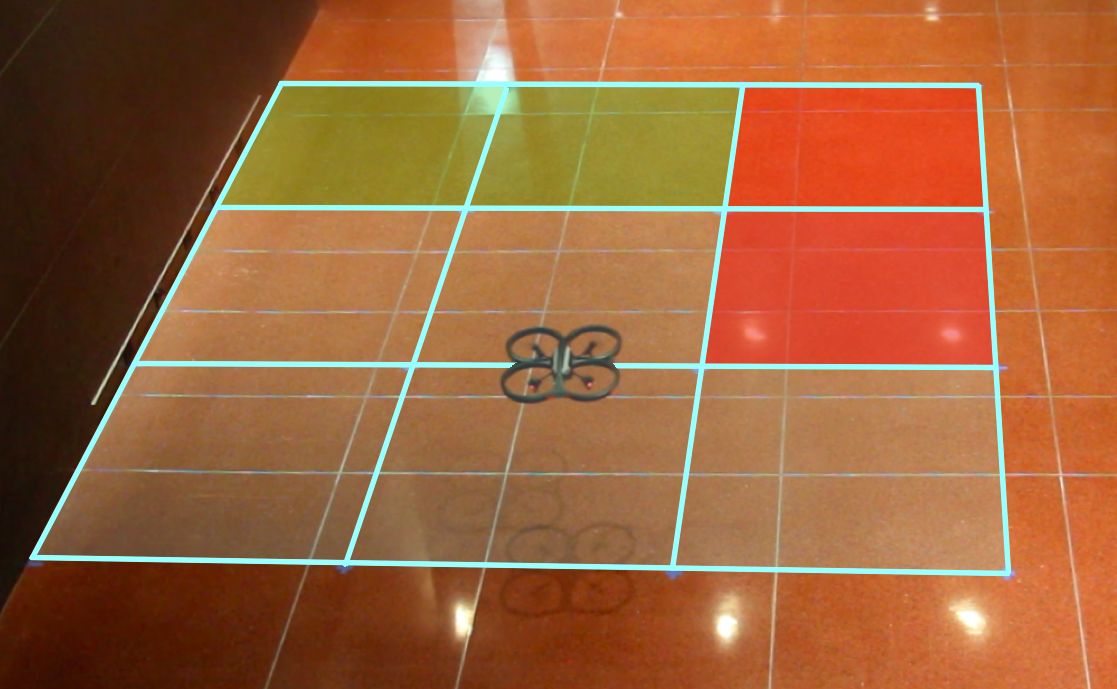
\includegraphics[scale=.2]{figure1}
  \caption{Three TurtleBots on a grid-based map each attempt to reach the goal zones (green) on the map while avoiding the danger zones (red).}
\end{figure}
\par
Importantly, redundancy is considered by utilizing N-1 sensor readings from other robots in addition to the sensors on each robot in order to estimate the state of each robot on a map. Problems such as the one posed in this paper can be solved by MDPs. MDPs can be applied to many other cyber-physical systems that utilize multiple sensor measurements to make a prediction of state according to optimal policy. A particle filter is applied in order to reasonably estimate where a robot using this system is located based on the optimal policy determined by the ROMDP given the N sensor measurements of this robot from itself and co-operative robots.
\par
This paper contributes (1) slight modifications to the ROMDP algorithm proposed in [1], (2) a proposed technique to deal with up to N-1 terrorized robots each with sensors measuring their own and other robot locations using ROMDP paired with a particle filter, and (3) simulation and experimental results important to evaluate the usability of this method in real-world scenarios considering mobile robots with monitoring allies.
\par
Following, the paper is organized like so: Section 2 describes work related to the method proposed; Section 3 formally defines the problem being investigated; Section 4.1 covers the details the ROMDP algorithm and any modifications made; Section 4.2 details the generic particle filter algorithm; Section 4.3 outlines the positional state estimation technique proposed using ROMDP and the generic particle filter; Section 5 covers the simulation outline, process and experimental results of a robot with terrorized sensors and 2 non-terrorized co-operatives. Lastly, section 6 concludes the paper and future work is discussed.
% end of introduction

% start of related work
\section{Related Work}

% end of related work

% start of problem
\section{Problem Formulation}

% end of problem


% start robot predict
\section{Using Multiple Robot Sensors to Predict the Location of a Single Mobile Robot}

% start ROMDP
\subsection{Redundant Observable Markov Decision Processes}

% end ROMDP

% start particle filter
\subsection{Generic Particle Filter}
% end particle filter

% start robot technique
\subsection{Estimating the Position of a Terrorized Robot using ROMDP and a Particle Filter}
% end robot technique

% end robot predict


% start robot case study
\section{TurtleBot Case Study}

% end robot case study


\section{Conclusion}
The conclusion goes here.

% use section* for acknowledgment
\section*{Acknowledgement}


The authors would like to thank...


% references section

% can use a bibliography generated by BibTeX as a .bbl file
% BibTeX documentation can be easily obtained at:
% http://mirror.ctan.org/biblio/bibtex/contrib/doc/
% The IEEEtran BibTeX style support page is at:
% http://www.michaelshell.org/tex/ieeetran/bibtex/
%\bibliographystyle{IEEEtran}
% argument is your BibTeX string definitions and bibliography database(s)
%\bibliography{IEEEabrv,../bib/paper}
%
% <OR> manually copy in the resultant .bbl file
% set second argument of \begin to the number of references
% (used to reserve space for the reference number labels box)
\begin{thebibliography}{1}

\bibitem{IEEEhowto:kopka}
Bezzo, N. et al. \emph{A Guide to \LaTeX}, 3rd~ed.\hskip 1em plus
  0.5em minus 0.4em\relax Harlow, England: Addison-Wesley, 1999.

\end{thebibliography}




% that's all folks
\end{document}